%\usepackage{pstricks}

\documentclass[a4paper, 12pt]{article}
\usepackage[utf8]{inputenc}
\usepackage{graphicx}
\usepackage{amsmath}

\title{COMP6212 Assignment 1}
\author{Junjun Shi}
\renewcommand{\thesubsection}{\thesection.\alph{subsection}}



\begin{document}

    \maketitle

	\section{Efficient Mean-Variance frontier}

	\subsection{}
    
    Generate 100 random portfolios and plot their expected return and variance. 

    The whole procedure could be described as:
    \begin{itemize}
        \item Construct 100 vectors X whose length is 3, and the elements $x_1,x_2,x_3$ satisfy $\sum\limits_{i=1}^{3} x_i= 1$ and $x_i\geq 0$ .
		\item For each vector:
		\begin{itemize}
			\item Calculate the expected return $E = \sum_{i=1}^3 X_i \mu_i$,
		    \item Calculate the expected variance $V = \sum_{i=1}^3 \sum_{j=1}^3 X_i X_j \sigma_{ij}$.
		\end{itemize}
    \end{itemize}
	Plot a scatter of diagram, we can get the picture like figure~\ref{fig:q1_a}.
	
	\begin{figure}
		\begin{center}
			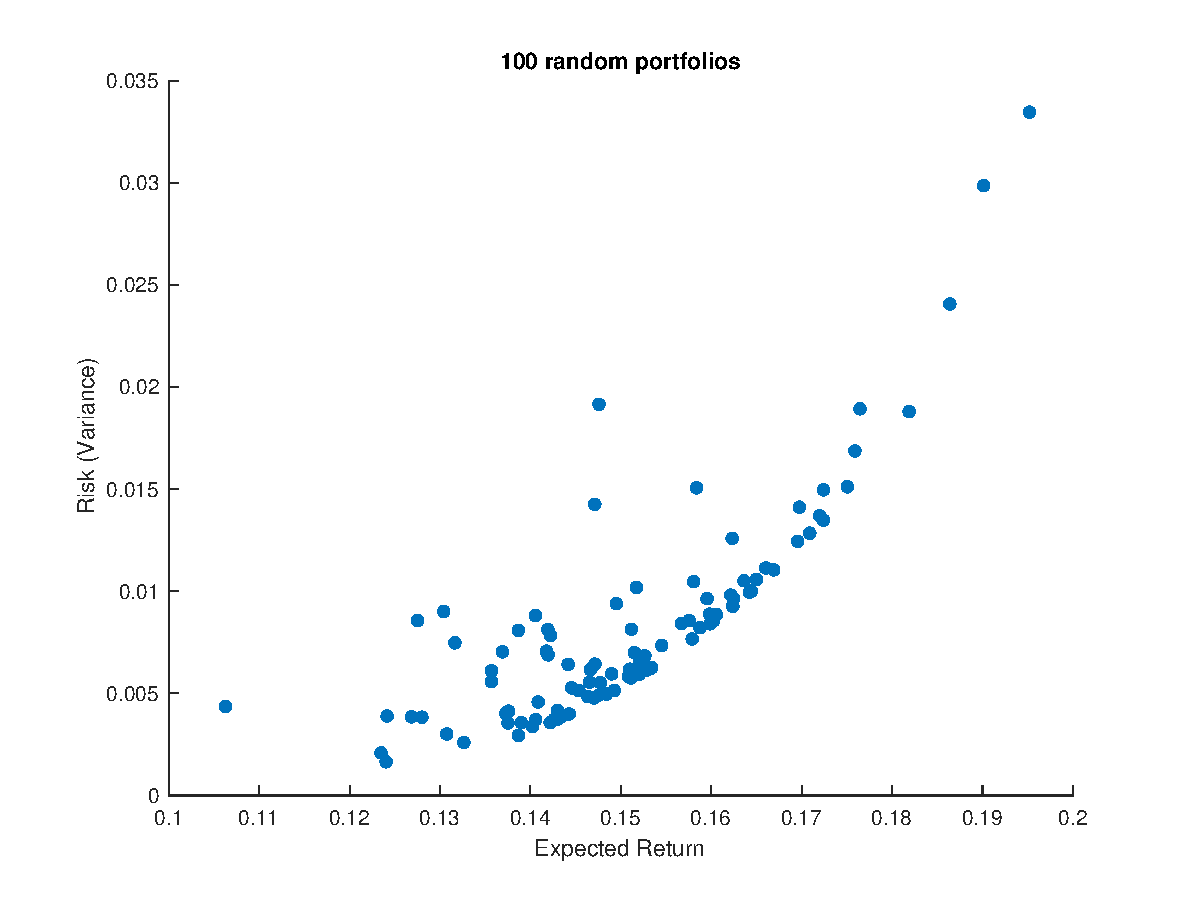
\includegraphics[width=0.85\linewidth]{q1_a.eps}
		\end{center}
		\caption{E-V plot of 100 randomly selected portfolios}
		\label{fig:q1_a}
	\end{figure}
	
	\subsection{}
	
	Matlab no longer support the function \texttt{frontcon} in version R2016b, I used the \texttt{Portfolio} object as replacement according to the offical documnetation.
	\begin{figure}
		\begin{center}
		    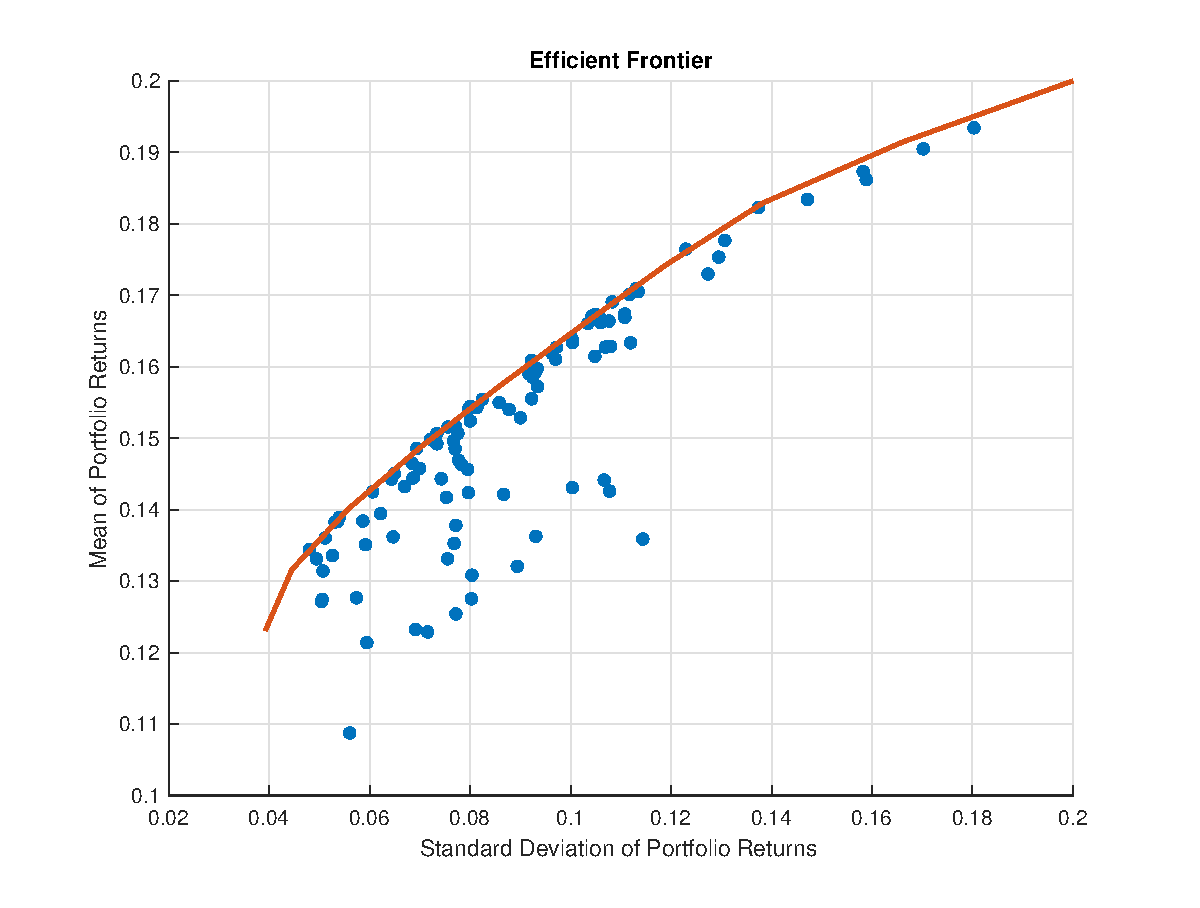
\includegraphics[width=0.85\linewidth]{q1_b_1.eps}
		\end{center}
		\caption{Efficient frontier for three-asset model}
		\label{fig:q1_b_1}
	\end{figure}
	
	From the figure~\ref{fig:q1_b_1} we can find that the \texttt{frontier} gives a left bound of portfolios. 
	
	\begin{figure}
		\begin{center}
       		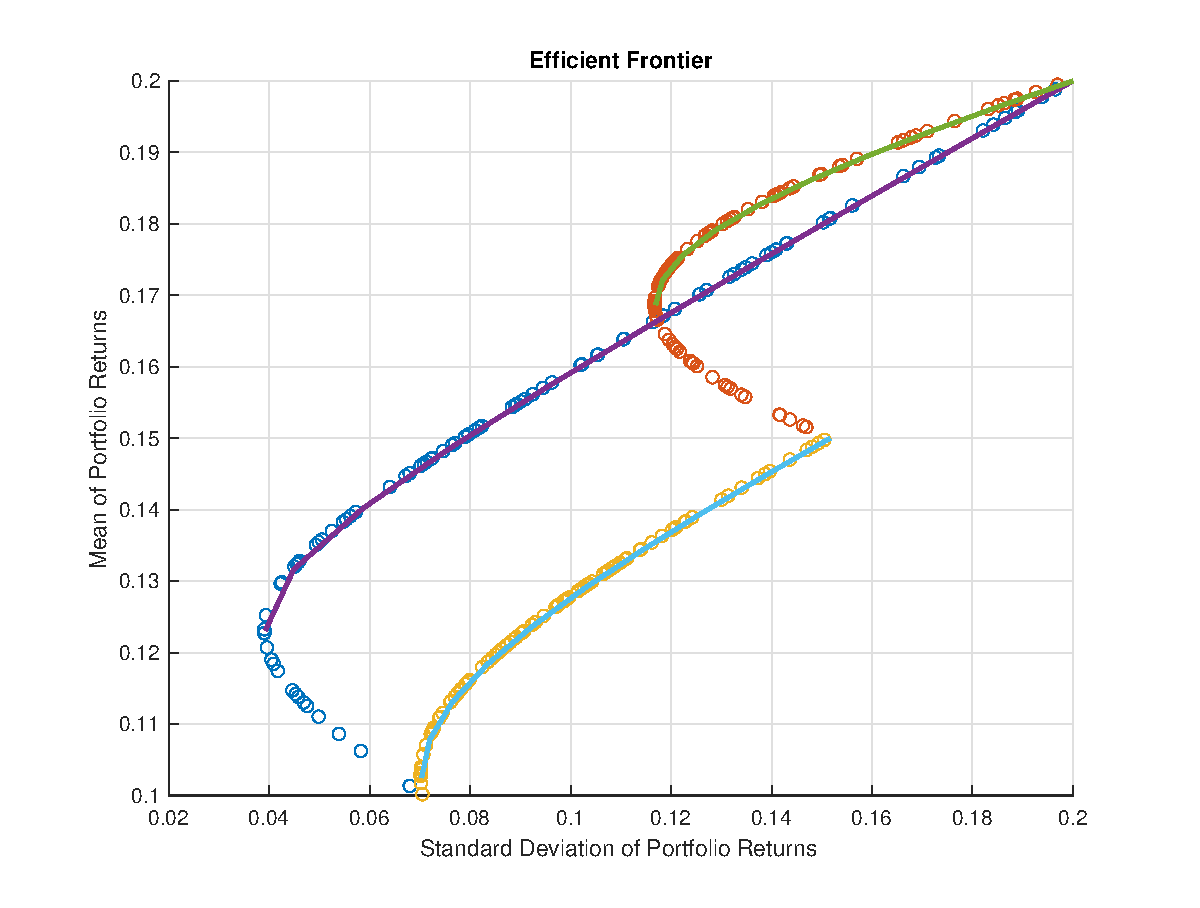
\includegraphics[width=0.85\linewidth]{q1_b_2.eps}
		\end{center}
		\caption{Efficient frontiers for two-asset models}
   		\label{fig:q1_b_2}
	\end{figure}
	
	The figure~\ref{fig:q1_b_2} shows the three two-asset models, the all exist on a single line, and the frontier is also part of the line.

	
	\subsection{}
	The \texttt{NativeMV} function claculate the status of Maximum return and Minimum risk, divide the range of return accroding to the given number, and calculate the minimum risk of each state. The \texttt{linprog} function is used by \texttt{NativeMV} to find out the maximum return at first.
	
	The maximum problem:
	
	\[\text{max } \mathbf{w}^T \bar{\mathbf{r}} \text{ subject to } \sum_{i=1}^N w_i = 1, w_i \geq 0\]
	
	be rewritten as:
	
	\[\text{min } \textnormal{-}\mathbf{w}^T \bar{\mathbf{r}} \text{ subject to } \sum_{i=1}^N w_i = 1, w_i \geq 0\]
	
	to use the  \texttt{linprog} function to get the ansewer.
	
	\subsection{}
	The figure~\ref{fig:q1_d} shows the result of using original \texttt{NativeMV} with \texttt{linprog},\texttt{quadprog} and the result of using \texttt{CVX} are identical. This is because that the problem they are solving are identical, just using different methods. CVX is suitable for solving more generic problems. However, CVX cost much more time, which could be easily observed while running code.
	\begin{figure}
		\begin{center}
       		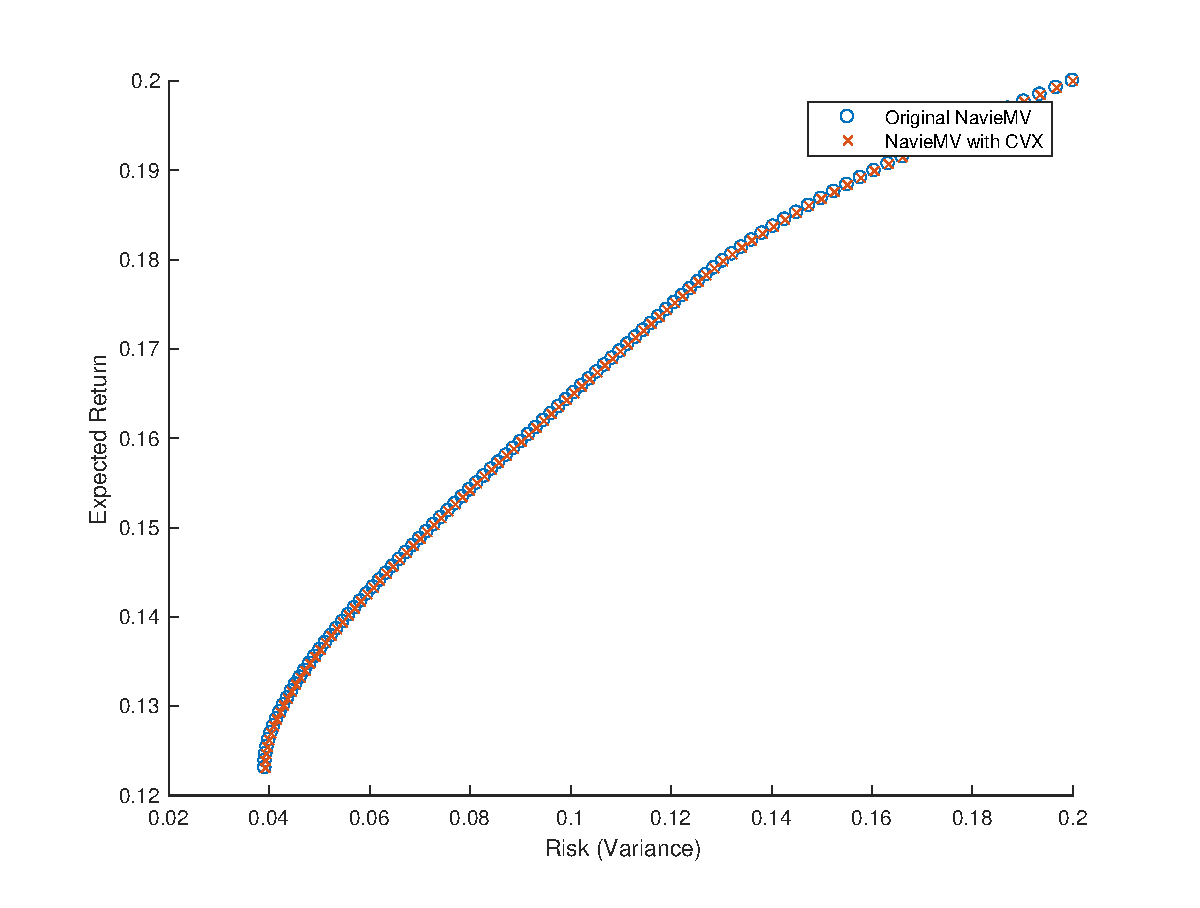
\includegraphics[width=0.85\linewidth]{q1_d.eps}
		\end{center}
		\caption{Performance of CVX}
   		\label{fig:q1_d}
	\end{figure}
	
	\section{Evaluation of performance}
	
	Downloaded the three-year data from \texttt{Yahoo! Finance}, using the close price to stand for the price of every single day, the days with no data are. For some situations like no transaction, I used the same price as the previous day standing for that day will have no retuen if you invest on it. Used MATLAB \texttt{tick2ret} function to get the return ratio.
	
	Calculated the mean retuen of the stocks got, and choosed three positive return stocks to do the next steps.
	
	Based on the data generated and the works done in \texttt{Question 1}, generate the frontier of the portfolios. Using the function \texttt{estimateFrontier} get a set of efficient portfolios and used \texttt{sharpe} function to find out the one with the hightest \texttt{Sharpe Ratio}.
	
	With the portfolio, we can compare it with the simple $\frac{1}{N}$ portfolio. As shown in the the figure~\ref{fig:q2}, the figure on the left represting daily return can not show which is better, for the \texttt{cumulative} one we can find that the efficient portfolio performs better than the navie one for a long window.
	\begin{figure}
		\begin{center}
       		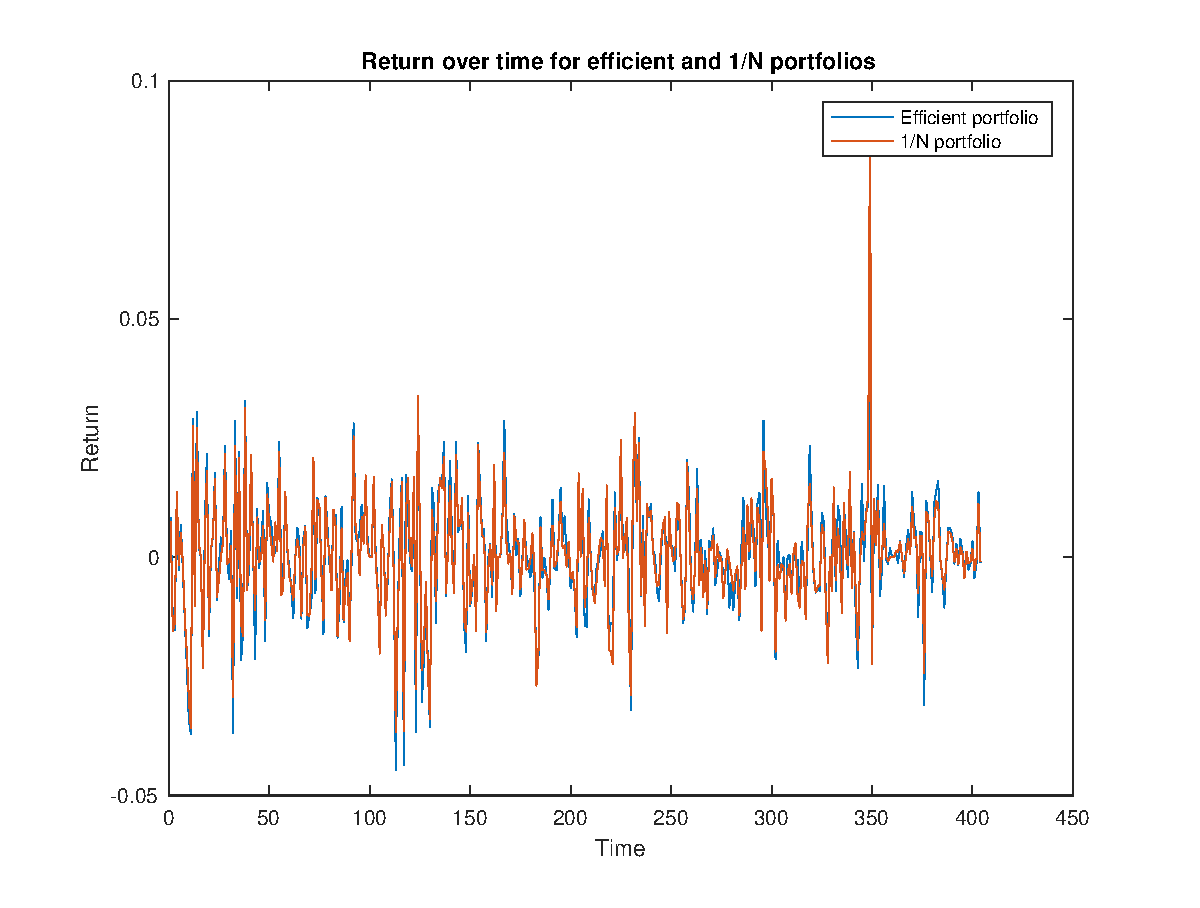
\includegraphics[width=0.45\linewidth]{stock_price/q2_1.eps}
       		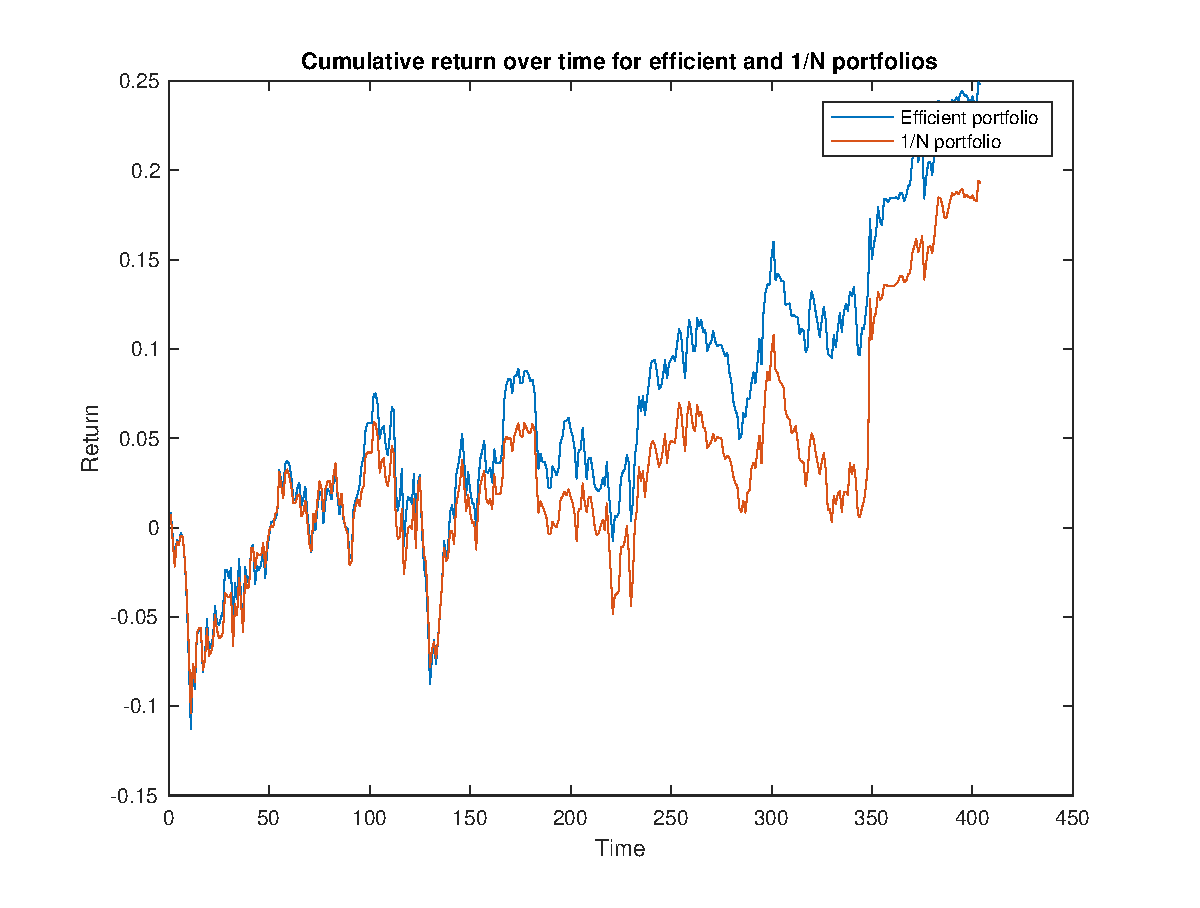
\includegraphics[width=0.45\linewidth]{stock_price/q2_2.eps}
		\end{center}
		\caption{Compare of Mean-Variance and Navie $\frac{1}{N}$ strategy}
   		\label{fig:q2}
	\end{figure}
	
	\section{Greedy and sparse index tracking}
	\subsection{}
	For the greedy strategy, get the stock with the smallest error. After that, continue finding the one which will give the smallest error when added by the exist set. Repeatly doing so until I have \texttt{seven} stocks in my basket(I have 35 stocks to view and one-fifth is 7).
	According the stocks selected are \texttt{4,7,11,13,16,18,27}. As the greedy search their weight are the same. The result of tracking is shown as figure~\ref{fig:q3_a}.
	\begin{figure}
		\begin{center}
       		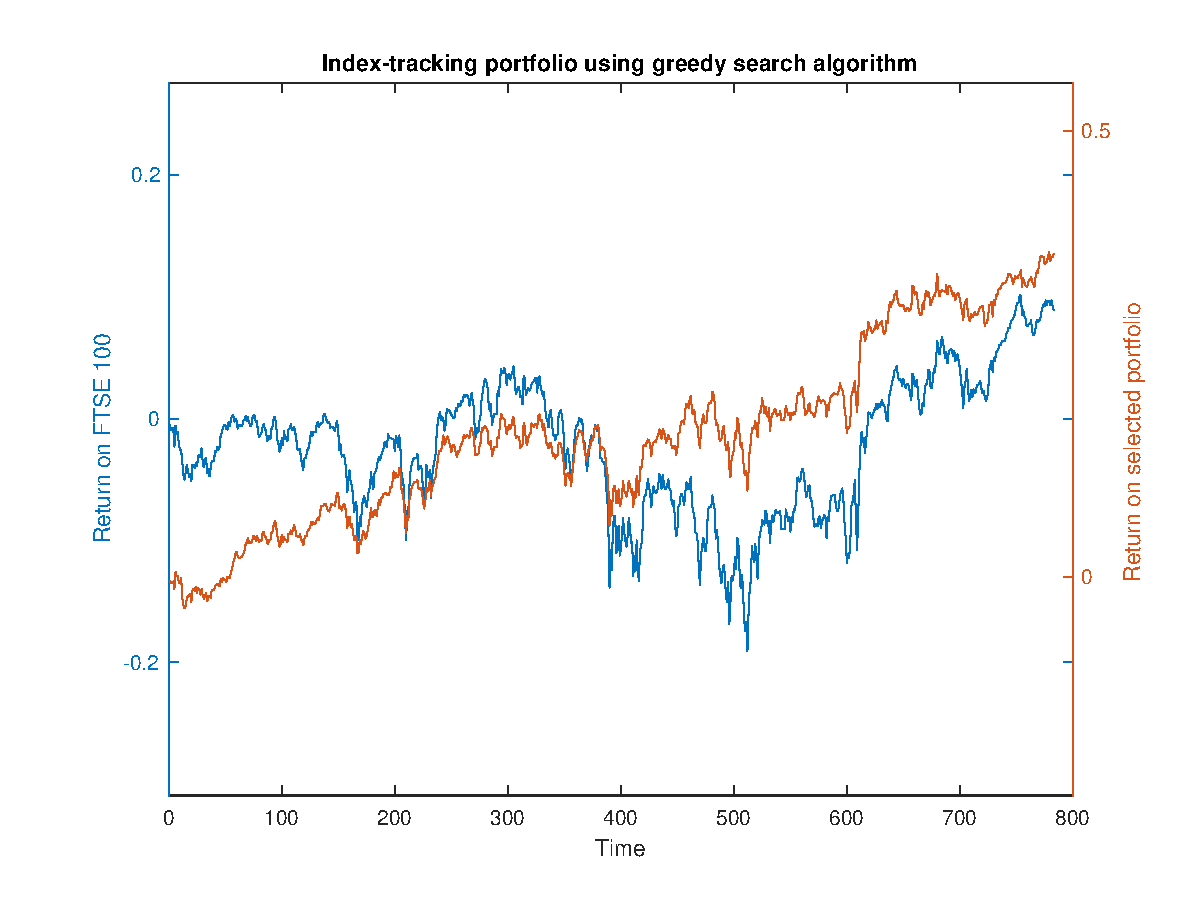
\includegraphics[width=0.45\linewidth]{stock_price/q3_a.eps}
		\end{center}
		\caption{Index tracking portfolio selected via greedy search}
   		\label{fig:q3_a}
	\end{figure}
	\subsection{}
	The second strategy to select stocks is to use index tracking algorithm to sole the problem:
	
	\[\mathbf{\hat{w}} = \min_{w} [\|\mathbf{y} - \mathbf{Rw}\|_2^2 \]
	
	To achieve a sparse result, using the technique of $L^1$-regularization. Use CVX toolkit to solve the problem:

	\[\mathbf{\hat{w}} = \min_{w} [\|\mathbf{y} - \mathbf{Rw}\|_2^2 + \tau \| \mathbf{w} \|_1]\]
	
    A value of $\tau = 0.1$ was selected to produce a 6 asset portfolio, whe result is shown in figure~\ref{fig:q3_b}. The stocks welected are \texttt{3,10,14,22,28}, which is totally different from greddy method.
		
	\begin{figure}
		\begin{center}
       		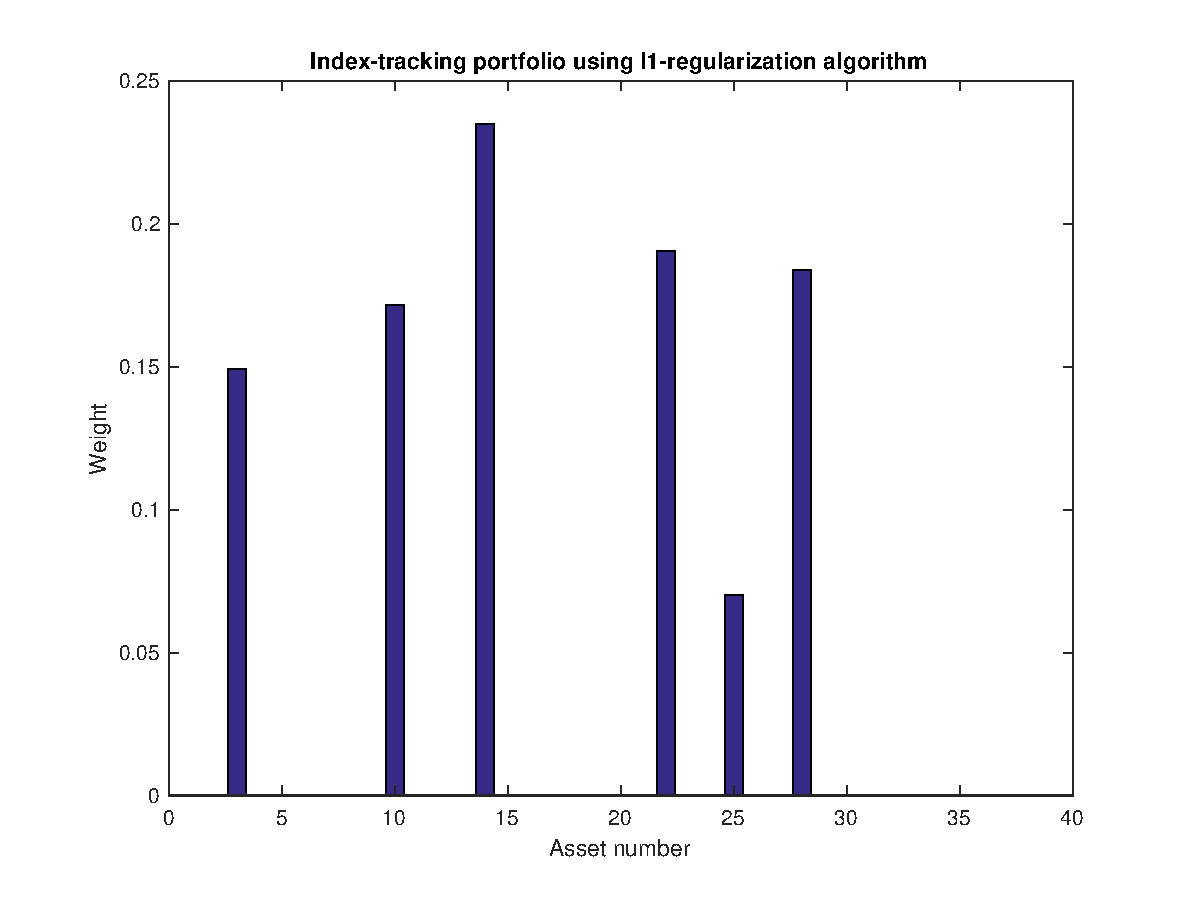
\includegraphics[width=0.45\linewidth]{stock_price/q3_b_1.eps}
       		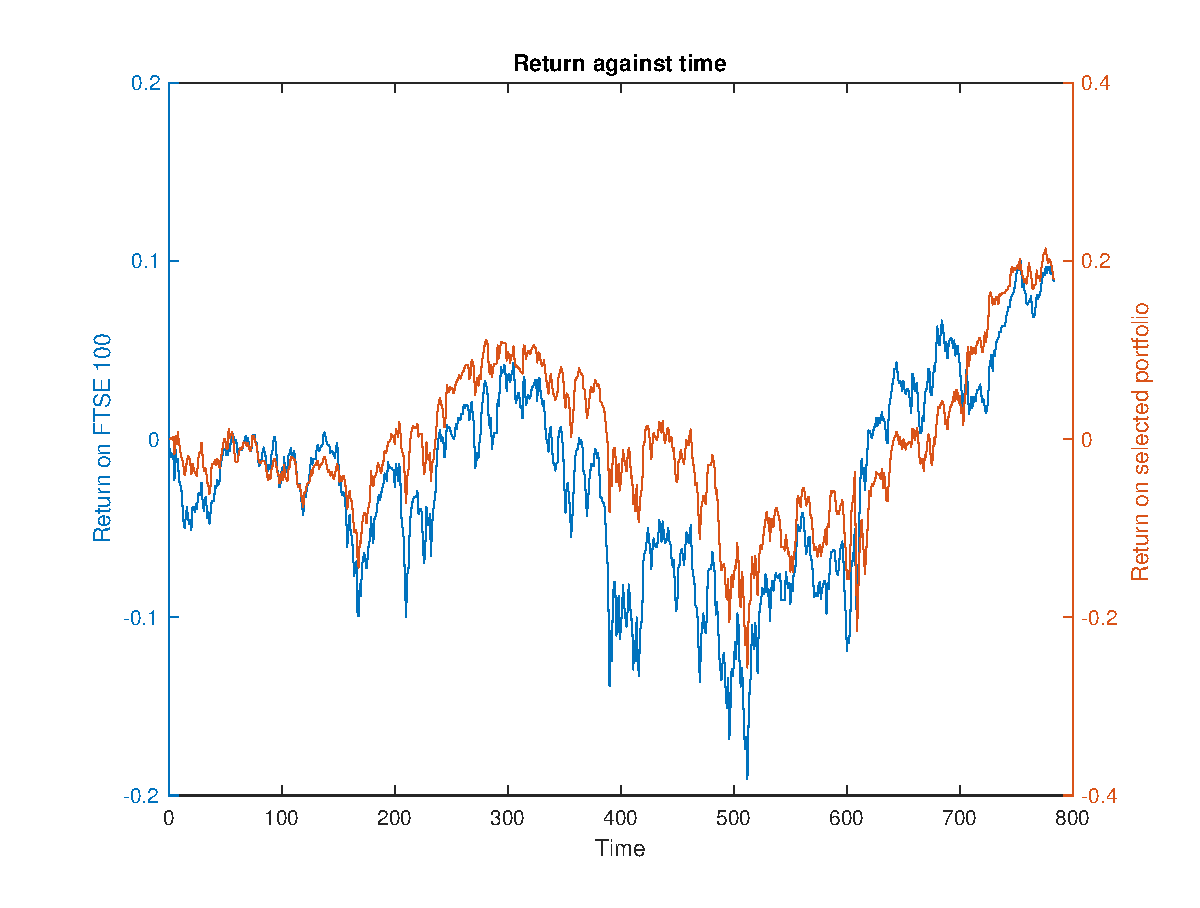
\includegraphics[width=0.45\linewidth]{stock_price/q3_b_2.eps}
		\end{center}
		\caption{Index tracking portfolio selected with $L^1$-regularization}
   		\label{fig:q3_b}
	\end{figure}
	 
	 To find a small number of stocks to invest and act as passive invester, we can find that the optimization method is more precise than the greedy method, it looks closer to the line of FTSE 100. 
	
	\section{Discussion of Lobo et al.}
	To analysis the transaction cost and how it will influence the portfolio, we use a new variable $x$, for a holding portfolio $w$, the new portfolio will be $w+x$. For an observed return of the assets $a=(a1 ... a2)$, we can get the mean $\bar{a}$ and the variance $\Sigma$.
	So we have an objective function:
	
	$$ maximize \qquad \bar{a}^T(w+x) $$
	
	And we have serval constraints on the function.

    \begin{itemize}
		\item The cost of transaction and buying new aseests should be covered by selling shares. ( $ 1^Tx+\phi(x)\leq 0$)
		\item Some rules based hobbies or experience. Like what's the maximum amount to invest.
		\item Money will be lost during transaction, a low bound is needed to limit the frequent shortselling. ($w_i+x_i\geq - s_i, i=1,...,n.$)
		\item The risk should not be too high. Setting an up bound for variance. ($(w+x)^T\Sigma(w+x)\leq\sigma_{max}$)
		\item If the return $a \sim \mathcal{N}(\bar{a},\,\Sigma)\,.$, the return will probably larger than a certain amount. ($Prob(W\geq W^{low}) \geq \eta$)
	\end{itemize}
	
	According to this rules, we can write CVX's constraints to use CVX solve the optimization problem in an acceptable time.	
	
	



\end{document}